All the technologies for data-centric governance exist and are aligned to simultaneously make better products with more socially beneficial outcomes. What is missing at present is the organizational capacity to build and maintain the tests and requirements. While this can and should be done within the same organizations that are creating the products, there is a real concern that organizations seeking to rapidly deploy products to capture markets will exert pressure on evaluation teams to certify those products prematurely.

While such potential conflicts of interest exist in many fields, they are especially acute in data-driven AI because publicly releasing the data needed to evaluate the system destroys the data's validity as an evaluation tool. Unlike, for example, automobile crash testing, where it would be very difficult to ``cheat'' a properly constructed test, in AI it is often trivial to achieve high performance on any given evaluation simply by training on the test data. 

These considerations prompt us to advocate for the establishment of \emph{evaluation authorities} -- independent entities that perform data-driven evaluations as a service and who accept responsibility for proper stewardship of the evaluation data. Such independent evaluation benefits both product developers and consumers. Product developers are protected from self-delusion due to biases in their internal evaluations, ultimately leading to better products, and they are perhaps also protected from legal liability as the evaluation authority's stamp of approval can provide evidence of due diligence in evaluating their products. Consumers benefit from objective standards by which they can compare products, analogous to crash safety ratings for automobiles or energy efficiency ratings for appliances.

In fact, a forerunner of the evaluation authorities and processes we envision already exists, under the umbrella of ``machine learning (ML) competitions.''

\textbf{What is an ML Competition?}

Machine learning is large field of research and engineering where many organizations routinely run billions of experiments. Consequently, the field is in statistical crises. With every experiment comes some probability that a high performing model got lucky instead of smart. Bringing order to the epistemological chaos is the machine learning competition, which sets competitors out to maximize some measure on private data not provided to the competing teams.

The most famous ML competition was ImageNet \cite{deng_imagenet_2009} for which academics were asked to produce a computer system capable of labeling image contents. In 2012 an entry into the multi-year competition vastly outperformed other entrants and produced a sea change in machine learning research. Figure \ref{fig:imagenet} depicts the rapid advancements on the ImageNet task.

\begin{figure}
     \centering
     \begin{subfigure}[b]{0.23\textwidth}
         \centering
         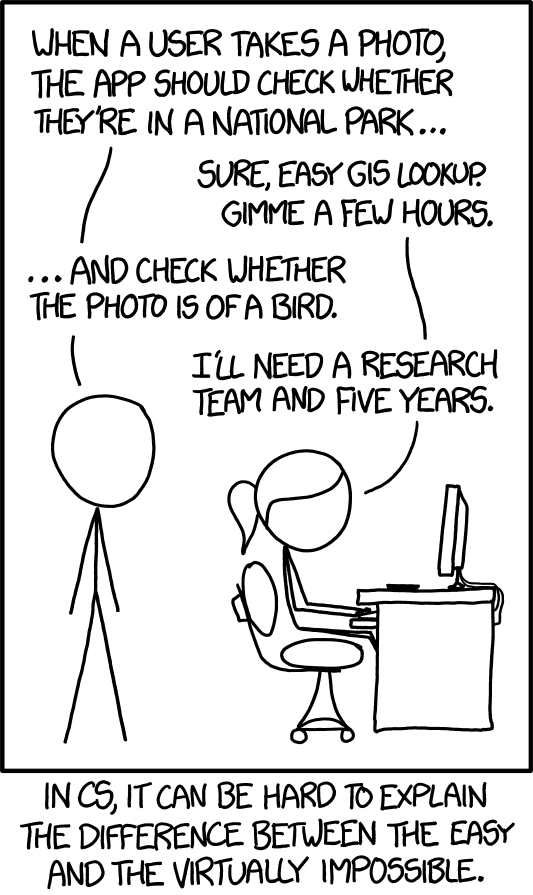
\includegraphics[width=\textwidth]{images/xkcd.png}
         \caption{The prevailing view of image classification prior to 2012 \cite{munroe_tasks_2014}.}
         \label{fig:xkcd}
     \end{subfigure}
    %  \hfill
    %  \begin{subfigure}[b]{0.49\textwidth}
    %      \centering
    %      \includegraphics[width=\textwidth]{images/ImageNet_hummingbird.jpeg}
    %      \caption{One example image from the ImageNet dataset of a hummingbird \cite{deng_imagenet_2009}. The complete dataset contains 1,000 different classified objects over a large image database.}
    %      \label{fig:humingbird}
    %  \end{subfigure}
    %  \hfill
     \begin{subfigure}[b]{0.76\textwidth}
         \centering
         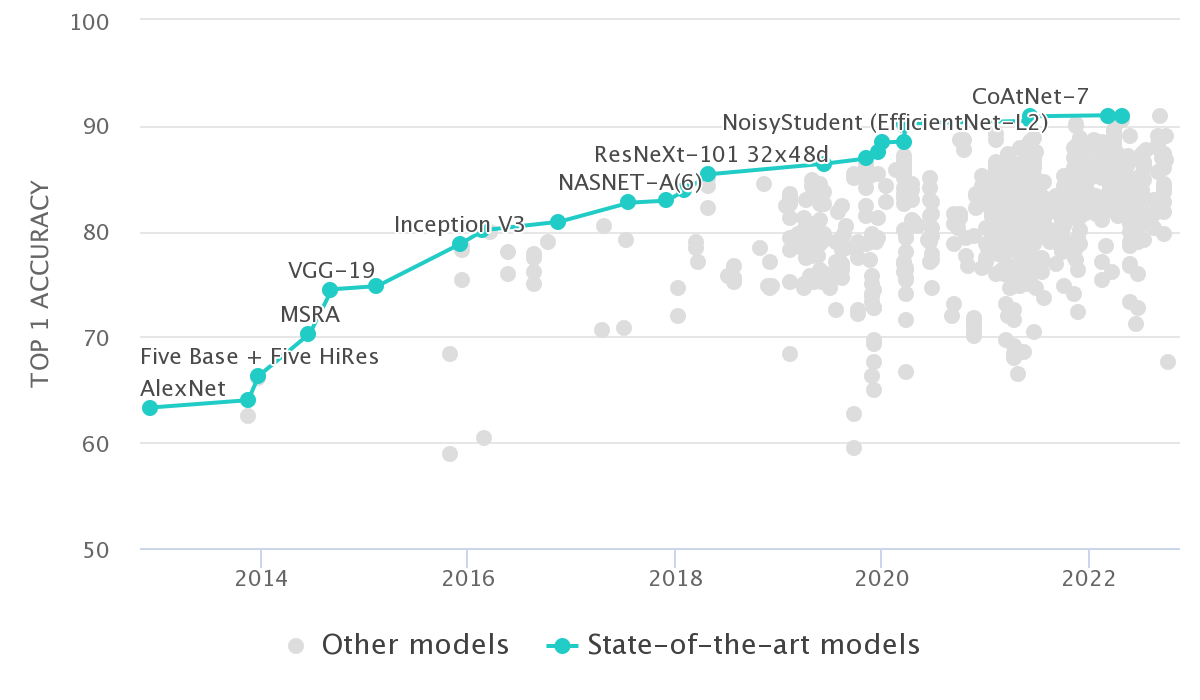
\includegraphics[width=\textwidth]{images/imagenet_benchmarks.png}
         \caption{Performance on the ImageNet test set through time \cite{robert_stojnic_papers_2022}.}
         \label{fig:imagenetbenchmarks}
     \end{subfigure}
     \caption{When the comic was published in 2014, we had just entered the most rapid period of improvement in computer vision systems then experienced. Recognizing a hummingbird in an image moved from hard to ``solved'' in the eyes of many machine learning researchers.}
     \label{fig:imagenet}
\end{figure}

By 2015, the prestige afforded to those besting the previous ImageNet leaders led a team of researchers to cheat on the competition \cite{simonite_why_2015}. The research team queried the private test set across multiple sham accounts to tune their model to the private test set. As a result, the performance estimates of the competition became invalid for the model and the researchers were banned from the competition.

\highlight{
\textbf{What can evaluation authorities tell us about system performance?}
Launched by Facebook in 2019, the Deepfake Detection Challenge \cite{dolhansky_deepfake_2019} looked to provide Facebook with tools that could detect computer-modified videos. While competitors made strong progress on the dataset Facebook filmed then modified in-house, the teams were ranked for a \$1,000,000 prize purse based on data from the platform's real users. Even though the user test data was not produced to circumvent detection, the degradation in performance between the Facebook-produced data and the Facebook user data as shown by Table \ref{tab:challengedata} is considerable. In effect, the competitors had produced models mostly capable of detecting when a face had been swapped, and not many other computer manipulations \cite{andrea_brennen_ai_2022}. Subsequent analysis also revealed the models regularly false activate for people with skin diseases, such as vitiligo.

\takeaway{Evaluation authorities have the ability to detect when systems are not robust}
}


\begin{table}
    \centering
    \begin{tabular}{|c|>{\centering\arraybackslash}p{0.55in}|>{\centering\arraybackslash}p{0.3in}|>{\centering\arraybackslash}p{0.55in}|>{\centering\arraybackslash}p{0.3in}|}
        \hline
         & \multicolumn{2}{c|}{Accuracy} & \multicolumn{2}{c|}{Ranking}  \\ \hline
         & Facebook-Generated Data & User Data & Facebook-Generated Data & User Data \\ \hline
         Competitor 1 & \roughly{}83\% & \roughly{}57\% & 1 & 905 \\ \hline
         Competitor 2 & \roughly{}82\% & \roughly{}65\% & 4 & 1 \\ \hline
    \end{tabular}
    \caption{ \textbf{Two competitor results from the Facebook Deepfake Detection Challenge.} All models degraded significantly from their test set performance on Facebook generated data to test set data defined on user generated data \cite{leibowicz_deepfake_2021}. }
    \label{tab:challengedata}
\end{table}

The practice of competitions serving as a form of evaluation authority has extended to the corporate world with organizations like the ML Commons \cite{ml_commons_mlcommons_2022}. Formed as an industry collaborative, ML Commons has 59 dues paying corporate members paying for evaluation datasets run by independent authorities. These evaluations historically were limited to simple properties such as accuracy, throughput, and energy, but the organization is increasingly integrating the evaluation and solution engineering steps to produce better performing systems across a wider array of performance attributes \cite{mazumder_dataperf_2022}. The benchmarking and engineering needs in the commercial sector are increasingly aligning to the principles of data-centric governance and filling the need for evaluation authorities. As shown in the next section, the scope of datasets needed to service the full variety of intelligent systems now under development in industry will require a great many organizations to form evaluation authorities.